

\section{Investigating perturbations of test problems with analytic solutions} \label{app:TestProblemsPerturbed}

As detailed in Section \ref{sec:Method_Solver}, it is necessary to provide an initial guess for the control $\vec{w}$ to start the optimization routine. Therefore, one method to validate the numerical method is to perturb the exact solution for $\vec{w}$ taken from a test problem with analytic solution and use this as an initial guess in the optimization solver. In the first iteration, the solutions for $\rho$ and $\adj$ differ from the exact solution. The optimization method then converges to the exact, optimal solution. We consider Test Problem 2 from Appendix \ref{app:TestProblems}, which is an exact solution for Problem \eqref{AdvDiff}, with boundary conditions \eqref{NoFlux}, and $\gamma = 0$. 
The following two perturbation functions are considered. The first perturbation is in time only and is defined as:
\begin{align*}
g(t) &= \frac{1}{2} f(t-t_0, a) \times f(t-t_0, -a)\\
&= \frac{1}{2} \frac{e^{-a/(t-t_0)}}{e^{-a/(t-t_0)} + e^{-a/(1-t -t_0)}} \times \frac{e^{a/(t-t_0)}}{e^{a/(t-t_0)} + e^{a/(1-t - t_0)}},
\end{align*}
and normalised by:
\begin{align*}
\tilde g(t) = \frac{g(t)}{\max{|{g(t)}|}}.
\end{align*}
A similar perturbation can be done in space, taking into account the difference in length of spatial and time domains:
\begin{align*}
h(x) &= \frac{1}{2} f(x-x_0, 2a) \times f(x-x_0, -2a)\\
&= \frac{1}{2} \frac{e^{-2a/(x-x_0)}}{e^{-2a/(x-x_0)} + e^{-2a/(1-x-x_0)}} \times \frac{e^{2a/(x-x_0)}}{e^{2a/(x-x_0)} + e^{2a/(1-x-x_0)}}.
\end{align*}
Again, this is normalised:
\begin{align*}
\tilde h(x) = \frac{h(x)}{\max{|{h(x)}|}}.
\end{align*}
These perturbation functions are chosen such that the perturbation is smooth and respects the initial condition for $\rho$, as well as the final time condition for $\adj$, by not changing the first or final time point. The considered perturbations are applied to the exact solution of the control, $\vec{w}_{ex}$, as follows:
\begin{align*}
\vec{w}_{pert1} &= \vec{w}_{ex}(1+ \epsilon \tilde g(t))\\
\vec{w}_{pert2} &= \vec{w}_{ex}(1+ \epsilon \tilde g(t) \tilde h(x)),
\end{align*}
where $a = 0.7$, $x_0 = t_0 = -0.01$ and the perturbation strength is either $\epsilon = 0.1$ or $\epsilon = 0.5$.
The chosen number of points is $N =30$ and $n=20$, the ODE tolerances are $10^{-8}$ and the optimality tolerance is $10^{-4}$. The mixing rate for the optimization solver is $\lambda = 0.01$.
The results presented in Table \ref{TabA2:Prob1} show the initial error in $\vec{w}$, $\mathcal{E}_{\vec{w}_{uc}}$, and the final errors in $\vec{w}$, $\rho$ and $\adj$, measured in the norm presented in Section \ref{sec:Method_Solver}, with respect to the exact solution. The initial error $\mathcal{E}_{\vec{w}_{uc}}$ is proportional to the perturbation strength $\epsilon$. The final errors for $\vec{w}$ and $\rho$ and $\adj$ are mostly within the specified optimality tolerance regardless of the perturbation strength and location. 

\begin{table}
\begin{tabular}{ | c | c || c | c | c | c ||}
\hline
  \multicolumn{2}{|c||}{} & $\beta = 10^{-3}$ & $\beta = 10^{-1}$ & $\beta = 10^{1}$ & $\beta = 10^{3}$  \\
\hline
\hline
\multirow{4}{*}{$0.1 \tilde g(t)$} & $\mathcal{E}_{\mathbf{w}_{uc}}$ & $\numprint{1.0000e-1}$ & $\numprint{1.0000e-1}$ & $\numprint{1.0000e-1}$ & $\numprint{1.0000e-1}$ \\
 & $\mathcal{E}_{\mathbf{w}_c}$ & $\numprint{5.3770e-5}$ & $\numprint{5.2340e-5}$ & $\numprint{5.2201e-5}$ & $\numprint{5.2203e-5}$ \\
 & $\mathcal{E}_{\rho}$ & $\numprint{1.1396e-5}$ & $\numprint{7.8597e-5}$ & $\numprint{7.8595e-5}$ & $\numprint{7.8597e-5}$ \\
 & $\mathcal{E}_{\adj}$ & $\numprint{2.7854e-5}$ & $\numprint{2.7836e-4}$ & $\numprint{5.7043e-4}$ & $\numprint{5.7045e-4}$ \\
\hline
\multirow{4}{*}{$0.5 \tilde g(t)$} & $\mathcal{E}_{\mathbf{w}_{uc}}$ & $\numprint{5.0000e-1}$ & $\numprint{5.0000e-1}$ & $\numprint{5.0000e-1}$ & $\numprint{5.0000e-1}$ \\
 & $\mathcal{E}_{\mathbf{w}_c}$ & $\numprint{2.1970e-4}$ & $\numprint{2.1747e-4}$ & $\numprint{2.1735e-4}$ & $\numprint{2.1735e-4}$ \\
 & $\mathcal{E}_{\rho}$ & $\numprint{2.4256e-5}$ & $\numprint{2.2878e-4}$ & $\numprint{2.2878e-4}$ & $\numprint{2.2879e-4}$ \\
 & $\mathcal{E}_{\adj}$ & $\numprint{3.3247e-5}$ & $\numprint{3.3227e-4}$ & $\numprint{6.8088e-4}$ & $\numprint{6.8090e-4}$ \\
\hline
\multirow{4}{*}{$0.1 \tilde h(x)$} & $\mathcal{E}_{\mathbf{w}_{uc}}$ & $\numprint{8.5568e-2}$ & $\numprint{8.5568e-2}$ & $\numprint{8.5568e-2}$ & $\numprint{8.5568e-2}$ \\
 & $\mathcal{E}_{\mathbf{w}_c}$ & $\numprint{5.3700e-5}$ & $\numprint{5.2250e-5}$ & $\numprint{5.2100e-5}$ & $\numprint{5.2103e-5}$ \\
 & $\mathcal{E}_{\rho}$ & $\numprint{1.1704e-5}$ & $\numprint{7.7973e-5}$ & $\numprint{7.7969e-5}$ & $\numprint{7.7968e-5}$ \\
 & $\mathcal{E}_{\adj}$ & $\numprint{2.6426e-5}$ & $\numprint{2.6387e-4}$ & $\numprint{5.6982e-4}$ & $\numprint{5.6984e-4}$ \\
\hline
\multirow{4}{*}{$0.5 \tilde h(x)$} & $\mathcal{E}_{\mathbf{w}_{uc}}$ & $\numprint{4.2784e-1}$ & $\numprint{4.2784e-1}$ & $\numprint{4.2784e-1}$ & $\numprint{4.2784e-1}$ \\
 & $\mathcal{E}_{\mathbf{w}_c}$ & $\numprint{2.1203e-4}$ & $\numprint{2.0982e-4}$ & $\numprint{2.0967e-4}$ & $\numprint{2.0968e-4}$ \\
 & $\mathcal{E}_{\rho}$ & $\numprint{2.2565e-5}$ & $\numprint{2.1275e-4}$ & $\numprint{2.1274e-4}$ & $\numprint{2.1275e-4}$ \\
 & $\mathcal{E}_{\adj}$ & $\numprint{3.0225e-5}$ & $\numprint{3.0219e-4}$ & $\numprint{6.1920e-4}$ & $\numprint{6.1923e-4}$ \\
\hline
\end{tabular}
\caption{Error measures for $\mathbf{w}_{uc}$, $\mathbf{w}_{c}$, $\rho$, and $\adj$, for four perturbation strategies for $\mathbf{w}$, and a range of $\beta$.}
\label{TabA2:Prob1}
\end{table} %\label{TabA2:Prob1}

%\begin{figure}[h]
%	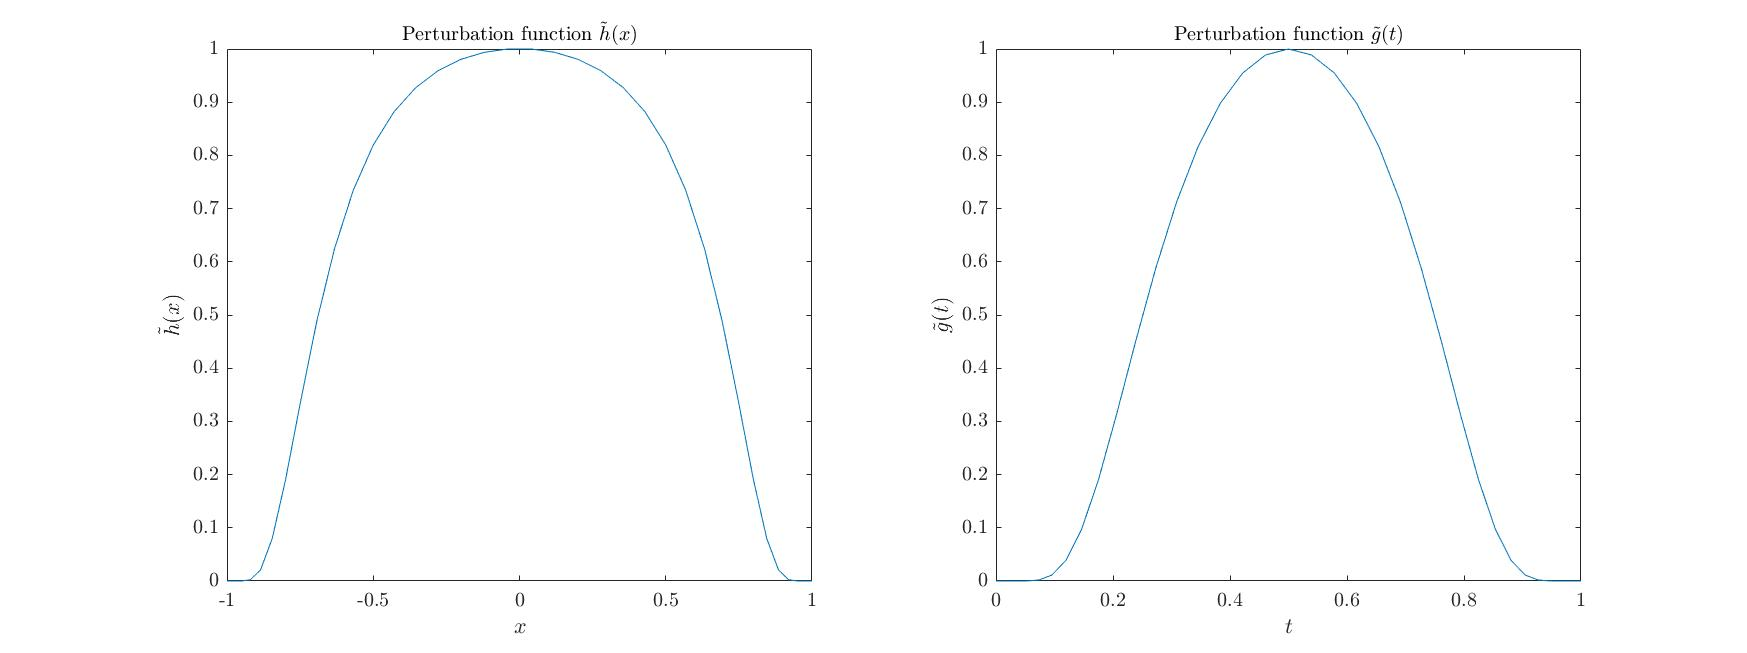
\includegraphics[scale=0.25]{PerturbationFunctions.jpg}
%	\caption{Perturbation functions $\tilde h(x)$ and  $\tilde g(t)$}
%	\label{Fig:PerturbationFunctions}
%\end{figure} 
%\begin{table}
%	\begin{tabular}{ ||c |c || c || c |c | c ||}
%		\hline
%		                    &	& Initial Error  & Final & Error &  \\ 
%		                	& $\beta$  & $\vec{w}$  & $\vec{w}$  & $\rho$ & $\adj$ \\ 
%		\hline
%			                & $10^{-3}$	& $0.1$  & $6.3190 \times 10^{-5}$ & $1.1648 \times 10^{-5}$ & $2.8425 \times 10^{-5}$  \\
%		 $0.1\tilde g(t)$   & $10^{-1}$	& $0.1$  & $6.1449 \times 10^{-5}$ & $7.9587 \times 10^{-5}$ & $2.8405 \times 10^{-4}$ \\
%		                 	& $10^{1}$	& $0.1$  & $6.1304 \times 10^{-5}$ & $7.9576 \times 10^{-5}$ & $5.8824 \times 10^{-4}$ \\
%		\hline 
%			                & $10^{-3}$	& $0.5$  & $2.7263 \times 10^{-4}$  & $2.9182 \times 10^{-5}$ & $3.2882 \times 10^{-5}$ \\
%		$0.5 \tilde g(t)$   & $10^{-1}$	& $0.5$  & $2.7064 \times 10^{-4}$ & $2.7098 \times 10^{-4}$ &  $3.2894 \times 10^{-4}$\\
%		                    & $10^{1}$	& $0.5$  & $2.7079 \times 10^{-4}$ & $2.7096 \times 10^{-4}$ & $6.8139 \times 10^{-4}$ \\
%		\hline 
%			                & $10^{-3}$	& $0.0855$ & $6.1809 \times 10^{-5}$ & $1.1842 \times 10^{-5}$ & $2.7355 \times 10^{-5}$ \\
%		$0.1\tilde h(x)$    & $10^{-1}$	& $0.0855$ & $6.0187 \times 10^{-5}$ & $8.0212 \times 10^{-5}$ & $2.7321 \times 10^{-4}$ \\
%		                    & $10^{1}$	& $0.0855$ & $6.0047 \times 10^{-5}$ & $8.0200 \times 10^{-5}$ & $5.7592 \times 10^{-4}$ \\
%		\hline 
%			                & $10^{-3}$	& $0.4276$  & $2.5041 \times 10^{-4}$ & $2.7429 \times 10^{-5}$ & $3.1303 \times 10^{-5}$ \\
%		$0.5\tilde h(x)$    & $10^{-1}$	& $0.4276$  & $2.4833 \times 10^{-4}$ & $2.5436 \times 10^{-4}$ & $3.1332 \times 10^{-4}$ \\
%	                     	& $10^{1}$	& $0.4276$  & $2.4846 \times 10^{-4}$ & $2.5435 \times 10^{-4}$ & $6.4922 \times 10^{-4}$ \\
%		\hline 
%    \end{tabular}
%	\caption{}
%\label{TabApp2}
%\end{table}
